\documentclass{beamer}

\usetheme{Berlin}
\usecolortheme{beaver}

\usepackage[utf8]{inputenc}
\usepackage[ngerman]{babel}
\usepackage{graphicx}
\usepackage{url} 
 
%Information to be included in the title page:
\title{Brust Krebs Diagnosis}
\author[]{Karla Araceli Luque Cobos, Maria Beatriz Walter Costa und Ulrike R\"osler \\ Betreuer: Anatol Reibold}
\institute{Big Data Analytics (alphatraining)}
\date{Oktober/2019}
 
\begin{document}
 
    \frame{\titlepage}

    \begin{frame}
    \frametitle{Hypothesis und Probleme}

    \begin{itemize}
    \item Hypothesis: es ist m\"oglich mit numerische Parametern Brustkrebs zu diagnostizieren (gut oder b\"oseartig)
    \item Problem I: Machine Learning models erstellen (von gut und b\"oseartige Stichproben)
    \item Problem II: neue Patientinnen klassifizieren (Diagnostics: g/b)
    \item Multivariate Dataset von 1995
            \begin{itemize}
            \item 569 Patientinnen
            \item 357 gutartige (63\%), 212 b\"osartige (37\%)
            \end{itemize}
    \end{itemize}
    \end{frame}
    
    \begin{frame}
    \frametitle{Dataset}

    \begin{itemize}
    \item Wie hat man dieser dataset gemacht?
    \item Krebs Brustzelle sammeln 
    \item Bilder auf Brustzellen machen (nuclei)
    \item Umsetzung von Bilder zu Parametern mit Image Recognition Methoden
    \item Output: Tabelle mit der numerische Parametern
    \item Source von University of Wisconsin (Kaggle): \url{https://www.kaggle.com/uciml/breast-cancer-wisconsin-data} 
    \end{itemize}
    \end{frame}

    \begin{frame}
    \frametitle{Parametern von der Tabelle}

    \begin{enumerate}
    \item ID number
    \item Diagnosis (M = malignant, B = benign)
    \item Ten real-valued features are computed for each cell nucleus:
        \begin{itemize}    
        \item a) radius (distance means from center to perimeter points)
        \item b) texture (std deviation of gray-scale values)
        \item c) perimeter
        \item d) area
        \item e) smoothness (local variation in radius lengths)
        \item f) compactness ($perimeter^2 / area - 1.0$)
        \item g) concavity (severity of concave portions of the contour)
        \item h) concave points (number of concave portions of the contour)
        \item i) symmetry
        \item j) fractal dimension (``coastline approximation'' - 1)
        \end{itemize}
    \end{enumerate}
    \end{frame}
    
    \begin{frame}
    \frametitle{Data Analysis (Pipeline)}
    \begin{figure}
    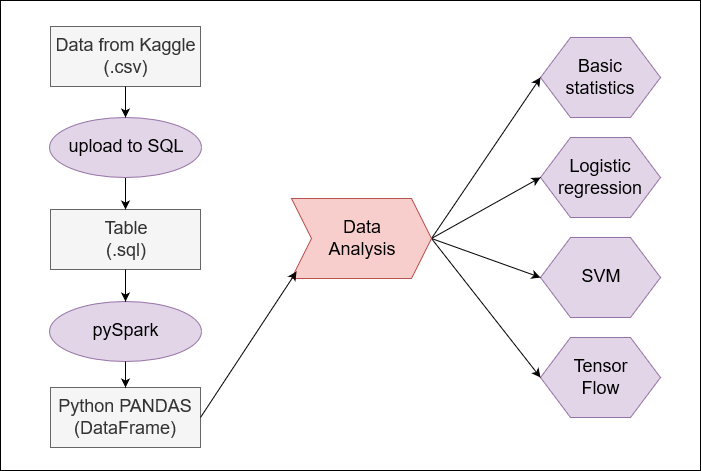
\includegraphics[width=0.85\columnwidth]{pipeline_cancer_project.png}
    \end{figure}
    \end{frame}
    
    \begin{frame}
    \frametitle{Ergebnisse}
    Python Jupyter Notebook:
    
    \url{http://localhost:8888/notebooks/Documents/Costa_MB/breast_cancer_diagnostics/jupyter_projekt.ipynb}
    \end{frame}

\end{document}


